\section{Design and Implementation}
\subsection{Power Stage Calculation and Component Selection}
Design of a 100W Forward Converter Operating in Continuous Conduction Mode (CCM) with
the following specifications:
\begin{table}[h!]
    \centering
    \begin{tabular}{ll}
        \toprule
        \textbf{Parameter} & \textbf{Value} \\
        \midrule
        Input Voltage ($V_{\text{in}}$) & $\SI{310}{\volt}$ \\
        Duty Cycle ($D$) & $30\% $ \\
        Output Voltage ($V_{\text{out}}$) & $\SI{24}{\volt}$ \\
        Diode Voltage $(V_d)$ & $1V$\\
        Output Power ($P_{\text{out}}$) & $\SI{500}{\watt}$ \\
        Switching Frequency ($f_{\text{sw}}$) & $\SI{100}{\kilo\hertz}$ \\
        Ripple Current Rated ($\Delta I_{\text{ripple}}$) & $30\%$ \\
        Ripple Voltage Rated ($\Delta V_{\text{ripple}}$) & $1\%$ \\
        Efficiency & $90\%$ \\
        \bottomrule
    \end{tabular}
    \caption{System Parameters}
    \label{tab:system_parameters}
\end{table}
\subsection{Power Stage Calculation}
\subsubsection*{Transformer Turn Ratio}
\[
\frac{N_p}{N_s} = \frac{V_{in} \cdot D}{V_{out} + V_f} = \frac{310 \cdot 0.3}{24 + 1} = 3.72
\]
\subsubsection*{Output Current}
\[
I_{out} = \frac{P_{out}}{V_{out}} = \frac{500}{24} \approx 20.83\ \text{A}
\]
\subsubsection*{Load Resistance}
\[
R_{\text{load}} = \frac{V_{out}}{I_{out}} = \frac{24}{20.83} \approx 1.152\ \Omega
\]
\subsubsection*{Input Power}
\[
P_{in} = \frac{P_{out}}{\eta} = \frac{500}{0.9} \approx 555.55\ \text{W} 
\]
\subsubsection*{Primary Average Current}
\[
I_{p\_avg} = \frac{P_{in}}{V_{in}} = \frac{555.55}{310} \approx 1.79\ \text{A}
\]
\subsubsection*{Primary Ripple Current}
\[
\Delta I_{L_{p}} = 0.3 \cdot I_{primary\_avg} = 0.3 \cdot 1.79 \approx 0.537\ \text{A}
\]
% \subsubsection*{Primary Maximum Current}
% \[
%     I_{primary\_max} = I_{primary\_avg} + \frac{\Delta I_{L_{primary}}}{2} \approx 0.412\ \text{A}
%  \]
% \subsubsection*{Primary Minimum Current}
% \[
% I_{primary\_min} = I_{primary\_avg} - \frac{\Delta I_{L_{primary}}}{2} \approx 0.304\ \text{A}
% \]
\subsubsection*{Primary rms Current}
\[
I_{p\_rms} = \frac{P_{in}}{V_{in} \cdot \sqrt{D}} = \frac{555.55}{310 \cdot \sqrt{0.3}} \approx 3.27 \text{A}
\]
\subsubsection*{Primary Inductance}
\[
L_p = \frac{V_{in} \cdot D}{\Delta I_{L_p} \cdot f_{sw}} = \frac{310 \cdot 0.3}{0.537 \cdot 10^5} \approx 1.7\ \text{mH}
\]
\subsubsection*{Reset Winding Inductance}
\[
L_{\text{reset}} = L_p = 1.7\ \text{mH}
\]
\subsubsection*{Secondary Inductance}
\[
L_s = L_p \cdot \left( \frac{N_s}{N_p} \right)^2 
= 1.7 \cdot \left( \frac{1}{3.72} \right)^2 \approx \boxed{0.125\,\text{mH}}
\]
\subsubsection*{Secondary Average Current}
\[
I_{secondary\_avg} = I_{out} = 20.83\text{A}
\]
\subsubsection*{Secondary rms Current}
\[
I_{s\_rms} = \frac{I_{out}}{\sqrt{2}} = \frac{20.83}{\sqrt{2}} \approx 14.73 \text{A}
\]
\subsubsection*{Ripple Output Current}
\[
\Delta I_o = 0.3 \cdot I_{out} = 0.3 \cdot 20.83 = 6.25 \text{A}
\]
\subsubsection*{Maximum Output Current}
\[
I_{o\_max} =  I_o + \frac{\Delta I_o}{2} = 20.83 + \frac{6.25}{2} = 23.95\ \text{A}
\]
\subsubsection*{Minimum Output Current}
\[
I_{o\_min} = I_o - \frac{\Delta I_o}{2} = 20.83 - \frac{6.25}{2} = 17.7\ \text{A}
\]
\subsubsection*{Output Inductor}
\[
L_o = \frac{(V_{out} + V_f)(1 - D)}{\Delta I_{L_o} \cdot f_{sw}} = \frac{25 \cdot 0.7}{6.25 \cdot 10^5} \approx 28\ \mu\text{H}
\]
\subsubsection*{Ripple Output Voltage}
\[
\Delta V_{\text{ripple}} = 0.01 \cdot V_{out} = 0.24\ \text{V}
\]
\subsubsection*{Output Capacitor}
\[
C_{out} = \frac{I_{out} \cdot D}{f_{sw} \cdot \Delta V_{\text{ripple}}} = \frac{20.83 \cdot 0.3}{100 \cdot 10^3 \cdot 0.24}\approx 260\ \mu\text{F}
\]
\subsubsection*{MOSFET Selection}
\begin{center}
    \begin{minipage}{0.4\textwidth}
        \centering
        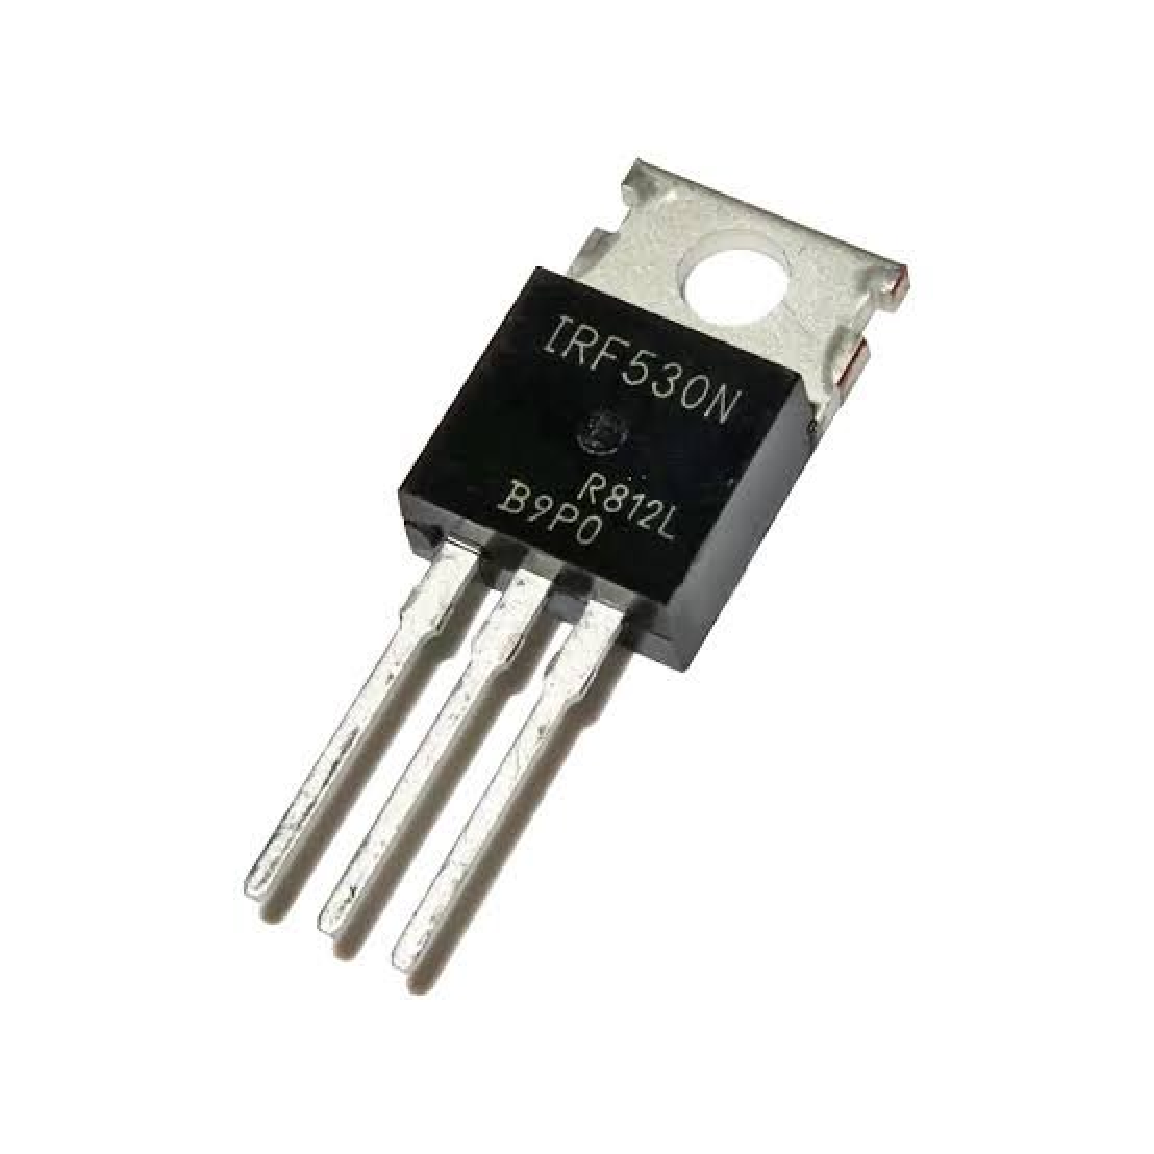
\includegraphics[width=0.8\linewidth]{Pictures/Images/mosfet.pdf} % Replace with your image file
        %\captionof{figure}{This is a figure.} % Add a caption
    \end{minipage}
    \hfill % Adds space between the minipages
    \begin{minipage}{0.55\textwidth}
    \centering
    \captionof{table}{STW11NM80 MOSFET}
    \label{tab:IRF530}
    \begin{tabular}{lcc}
    \toprule
    \footnotesize
    \textbf{Parameter} & \textbf{Value} & \textbf{Test Conditions} \\
    \midrule
     $V_{DS}$ & \SI{800}{\volt} & Absolute Maximum Rating \\
     $I_D$ & \SI{15}{\ampere} & $T_C = \SI{25}{\celsius}$ \\
     & \SI{10}{\ampere} & $T_C = \SI{100}{\celsius}$ \\
     $R_{DS(on)}$ & \SI{0.16}{\ohm} & $V_{GS} = \SI{10}{\volt}, I_D = \SI{8.4}{\ampere}$ \\
    \bottomrule
    \end{tabular}
    \end{minipage}
\end{center}
\subsubsection*{Diode Selection}
\begin{center}
    \begin{minipage}{0.4\textwidth}
        \centering
        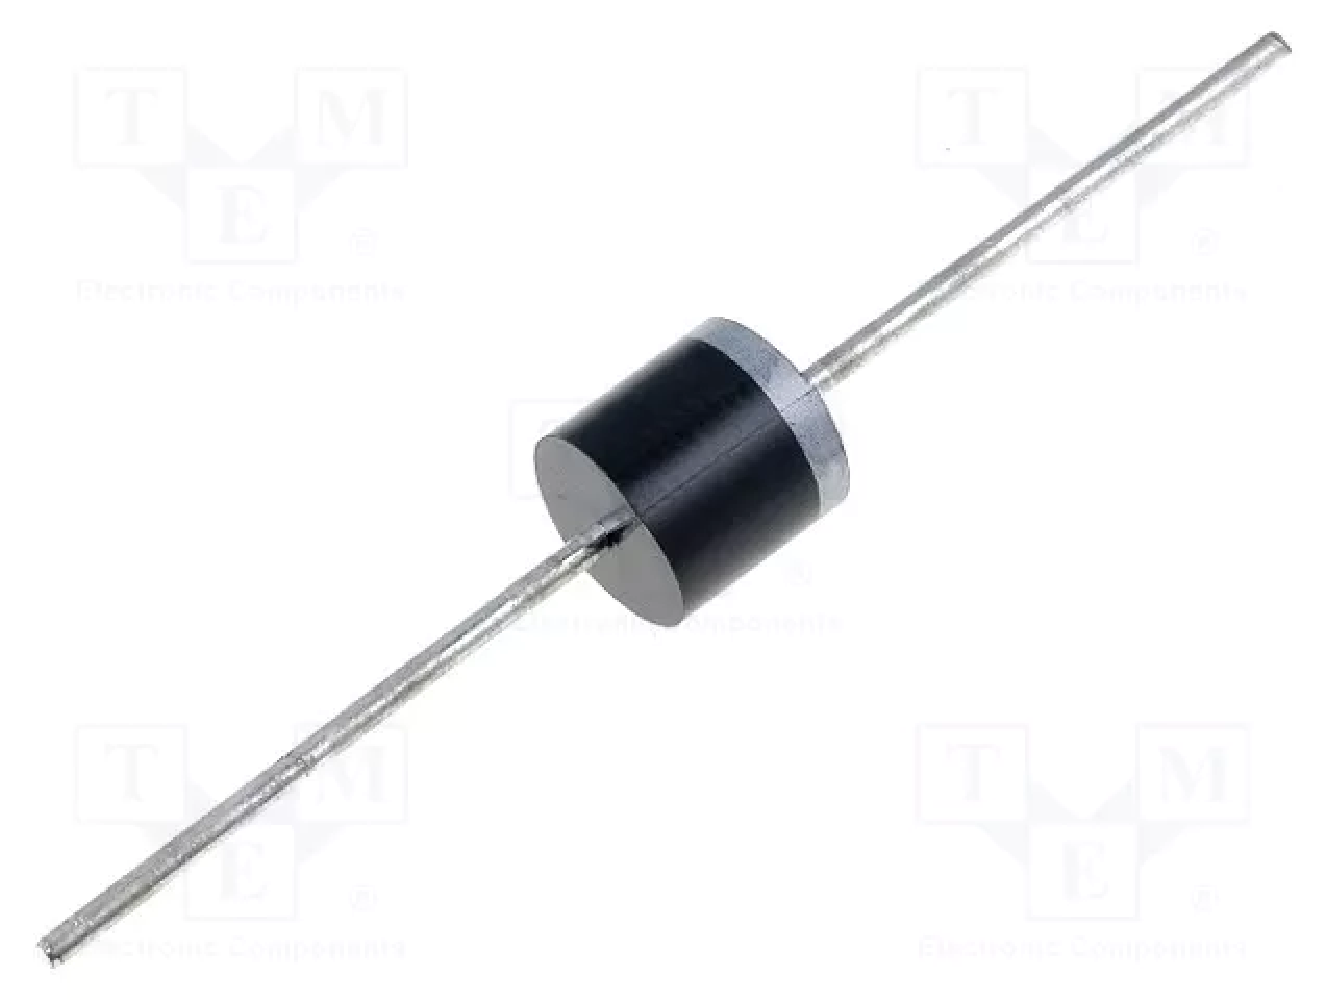
\includegraphics[width=0.7\linewidth]{Pictures/Images/diode.pdf} % Replace with your image file
        %\captionof{figure}{This is a figure.} % Add a caption
    \end{minipage}
    \hfill % Adds space between the minipages
    \begin{minipage}{0.55\textwidth}
    \centering
    \captionof{table}{VS-E5PX6012 Diode}
        \label{tab:SR510}
        \begin{tabular}{lcc}
        \toprule
        \textbf{Parameter} & \textbf{Value} & \textbf{Test Conditions} \\
        \midrule
        $V_{RRM}$ & \SI{1000}{\volt} & Maximum repetitive rating \\
        $I_F$ & \SI{50}{\ampere} & Continuous, $T_A = \SI{25}{\celsius}$ \\
        \bottomrule
        \end{tabular}
    \end{minipage}
\end{center}
\subsection{Transformer Design}
\begin{table}[h!]
\centering
\caption{Input Parameters for Forward Converter Design}
\label{tab:input_parameters}
\begin{tabular}{lccr}
\toprule
\textbf{Parameter} & \textbf{Symbol} & \textbf{Value} & \textbf{Unit} \\ 
\midrule
Input Power & \( P_{in} \) & \( 555.55\) & W \\ 
Switching Frequency & \( F \) & \( 100\) & kHZ \\ 
Ferrite Core Flux Density & \( B_m \) & 0.1 & T \\ 
Duty Cycle & \( D \) & 0.3 & - \\ 
Regulation Factor & \( \alpha \) & 0.5 & - \\ 
Primary RMS Current & \( I_{p,rms} \) & 3.27 & A \\ 
Secondary RMS Current & \( I_{s,rms} \) & 14.73 & A \\ 
\bottomrule`    
\end{tabular}
\end{table}
\subsubsection*{Electrical Coefficient }
\[
K_e = 0.145 \times F^2 \times B_m^2 \times 10^{-4} = 0.145 \cdot (10^5)^2 \cdot (0.1)^2 \cdot 10^{-4} = 1450
\]
\subsubsection*{Core Geometry}
\[
K_g = \frac{P_{in} \cdot D}{\alpha \cdot K_e}= \frac{555.55 \times 0.3}{0.5 \times 1450} \approx 0.2299\ cm^5
\]
\newpage
\begin{figure}[h!]
    \centering
    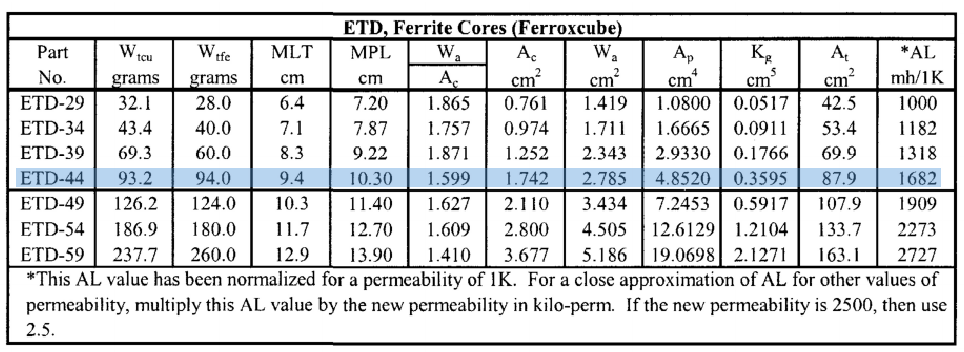
\includegraphics[width=1\linewidth]{Pictures/Images/ETD_CORE_500W.pdf}
    \caption{\textcolor{blue}{\textit{\footnotesize ETD Core Parameter Table List}}}
\end{figure} 
\begin{figure}[h!]
    \centering
    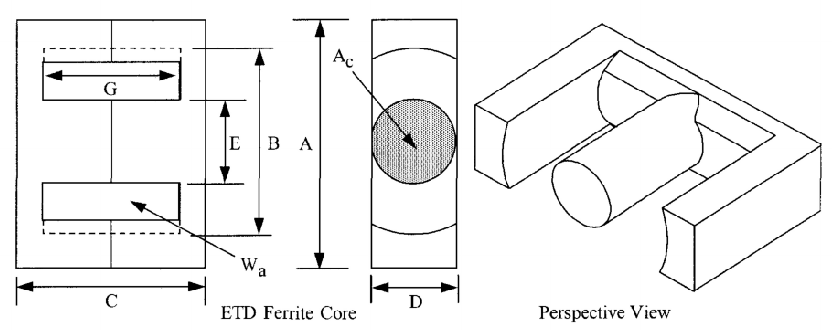
\includegraphics[width=0.8\linewidth]{Pictures/Images/ETD_CORE_STRUCTURE.pdf}
    \caption{\textcolor{blue}{\textit{\footnotesize ETD-29 Core}}}
\end{figure} 
\begin{table}[h!]
\centering
\begin{tabular}{l l l}
\toprule
\textbf{Parameter} & \textbf{Value} & \textbf{Unit} \\
\midrule
Magnetic Path Length ($MPL$) & $\SI{10.30}{}$ & \si{\centi\meter} \\
Core Weight ($W_{\text{core}}$) & $\SI{94}{}$ & \si{\gram} \\
Copper Weight ($W_{\text{copper}}$) & $\SI{93.2}{}$ & \si{\gram} \\
Mean Length Turn ($MLT$) & $\SI{9.4}{}$ & \si{\centi\meter} \\
Cross-Sectional Area ($A_c$) & $\SI{1.742}{}$ & \si{\centi\meter\squared} \\
Window Area ($W_a$) & $\SI{2.785}{}$ & \si{\centi\meter\squared} \\
Core Product ($A_p$) & $\SI{4.852}{}$ & \si{\centi\meter\tothe{4}} \\
Core Geometry ($K_{gs}$) & $\SI{0.3595}{}$ & \si{\centi\meter\tothe{5}} \\
\bottomrule
\end{tabular}
\caption{Selected Core Parameters for Transformer Design}
\label{tab:core_parameters}
\end{table}
\subsubsection*{Current Density (\(J\))}
\[
J = \frac{2 \cdot P_{\text{in}} \cdot \sqrt{D} \cdot 10^4}{F \cdot A_c \cdot B_m \cdot W_a \cdot K_u} = \frac{2 \cdot 555.55 \cdot \sqrt{0.3} \cdot 10^4}{10^5 \cdot 1.742 \cdot 0.1 \cdot 2.785 \cdot 0.4} = \SI{313.06}{\ampere\per\centi\meter\squared}
\]
\subsubsection*{Primary Bare Wire Area (\(A_{pw}\))}
\[
A_{pw} = \frac{I_{p,\text{rms}}}{J} = \frac{3.27}{282.2} = \SI{0.0104}{\centi\meter\squared}
\]
\subsubsection*{Primary Turns (\(N_p\))}
\[
N_p = \frac{V_{\text{in}} \cdot D \cdot 10^4}{F \cdot A_c \cdot B_m} =\frac{310 \cdot 0.3 \cdot 10^4}{10^5 \cdot 1.742 \cdot 0.1} = 53.38 \ \text{turns}
\]
\subsubsection*{Secondary Bare Wire Area (\(A_{sw}\))}
\[
A_{sw} = \frac{I_{s,\text{rms}}}{J} = \frac{14.73}{282.2} = \SI{0.047}{\centi\meter\squared}
\]
\subsubsection*{Secondary Turns (\(N_s\))}
\[
N_s = \frac{N_p \cdot (V_o + V_d)}{D \cdot V_{\text{in}}} = \frac{122 \cdot (24 + 1)}{0.3 \cdot 310} = 14.35\ \text{turns}
\]
\subsection{Output Inductor Design}
\begin{table}[h]
\centering
\caption{Design Specifications}
\begin{tabular}{lll}
\toprule
\textbf{Parameter} & \textbf{Symbol} & \textbf{Value} \\
\midrule
Inductance & $L$ & $28\ \mu$H \\
DC Current & $I_o$ & 20.83\ A \\
AC Current & $\Delta I$ & 6.25 A \\
Output Power & $P_o$ & 500\ W \\
Regulation & $\alpha$ & 1 \\
Ripple Frequency & $F_s$ & 100 kHz\\
Flux Density & $B_m$ & 0.25 T \\
Window Utilization & $K_u$ & 0.4 \\
Temperature Rise & $T_r$ & 25$^\circ$C \\
\bottomrule
\end{tabular}
\end{table}
\subsubsection*{Peak Current}
\[
I_{pk} = I_o + \frac{\Delta I}{2} = 20.83 + \frac{6.25}{2} = 23.95\ \text{A}
\]
\subsubsection*{Energy-Handling Capability}
\[
E = \frac{1}{2} L I_{pk}^2  = \frac{1}{2} \cdot 28\times 10^{-6} \cdot (23.95)^2 = 0.008\ \text{J}
\]
\subsubsection*{Electrical Coefficient}
\[
K_e = 0.145 \cdot P_o \cdot B_m^2 \cdot 10^{-4} = 0.145 \cdot 500 \cdot (0.25)^2 \cdot 10^{-4} = 0.00045313
\]
\subsubsection*{Core Geometry}
\[
K_g = \frac{E^2}{K_e \cdot \alpha} = \frac{(0.008)^2}{0.00045313 \cdot 1} = 0.1424\ \text{cm}^5
\]
\newpage
\begin{figure}[h!]
    \centering
    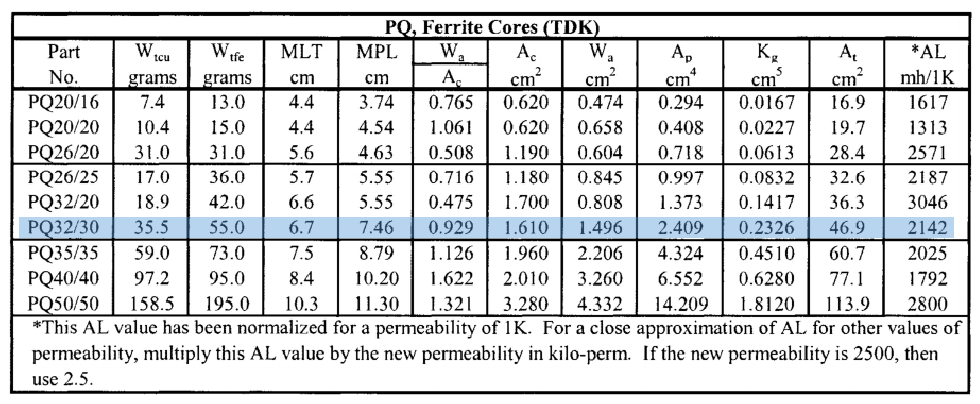
\includegraphics[width=1\linewidth]{Pictures/Images/PQ_CORE_500W.pdf}
    \caption{\textcolor{blue}{\textit{\footnotesize PQ Core Parameter Table List}}}
\end{figure} 
\begin{figure}[h!]
    \centering
    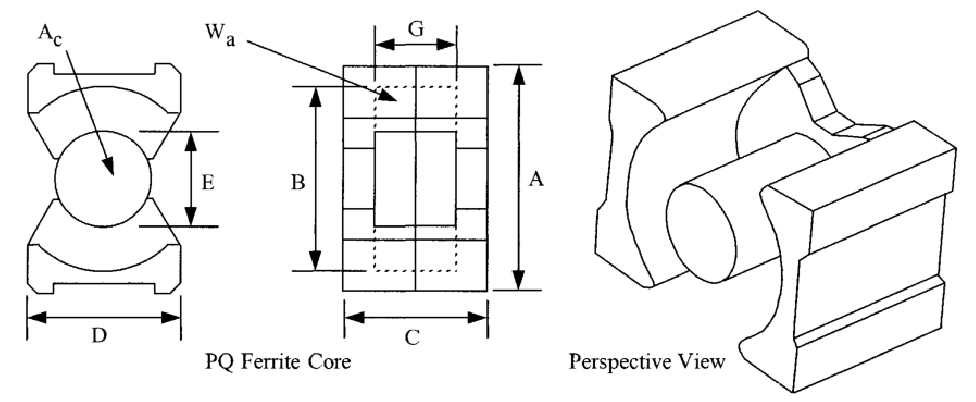
\includegraphics[width=0.8\linewidth]{Pictures/Images/PQ_CORE_STRUCTURE.pdf}
    \caption{\textcolor{blue}{\textit{\footnotesize PQ32/30 Core}}}
\end{figure} 
\subsubsection*{Current Density}
\[
J = \frac{2E \cdot 10^4}{B_m \cdot A_p \cdot K_u} = \frac{2 \cdot 0.008 \cdot 10^4}{0.25 \cdot 2.409 \cdot 0.4} = 664.176\ \text{A/cm}^2
\]
\subsubsection*{RMS Current}
\[
I_{rms} = \sqrt{I_o^2 + \left(\frac{\Delta I}{\sqrt{3}}\right)^2} = \sqrt{20.83^2 + \left(\frac{6.25}{\sqrt{3}}\right)^2} = 21.7474\ \text{A}
\]
\subsubsection*{Bare Wire Area}
\[
A_w = \frac{I_{rms}}{J} = \frac{21.7474}{664.1560} = 0.00608\ \text{cm}^2
\]
\subsubsection*{Selected Wire Area}
\[
A_{ws} = 0.035\ \text{cm}^2
\]
\subsubsection*{Effective Window Area}
\begin{itemize}
    \item $S_3 = 0.75$ Window Effective factor for Ferrite core
\end{itemize}
\[
W_{a,eff} = W_a \cdot S_3 = 1.496 \cdot 0.75 = 1.1220\ \text{cm}^2
\]
\subsubsection*{Number of Turn}
\begin{itemize}
    \item $S_2 = 0.6$ Fill Factor 
\end{itemize}
\[
N = \frac{W_{a,eff} \cdot S_2}{A_{ws}} = \frac{1.12 \cdot 0.6}{0.01} = 19.23\ \text{turns}
\]
\subsubsection*{Required Air Gap}
\[
L_g = \frac{0.4\pi N^2 A_c \cdot 10^{-8}}{L} - \frac{MPL}{\mu_0} = \frac{0.4\pi (19.23)^2 (1.61) \cdot 10^{-8}}{28 \times 10^{-6}} - \frac{7.46}{2500} = 0.12\ \text{cm}
\]
\subsection{Simulation on LTspice}
\begin{figure}[h!]
    \centering
    
\includegraphics[width=0.8\linewidth]{Pictures/Images/LT_schem.pdf}
    \caption{\textcolor{blue}{\textit{\footnotesize Forward Converter Schematic on LTspice}}}
\end{figure}
\begin{figure}[h!]
    \centering
    
\includegraphics[width=0.8\linewidth]{Pictures/Images/LT_output_voltage.pdf}
    \caption{\textcolor{blue}{\textit{\footnotesize Output Voltage Wave Form}}}
\end{figure}
\newpage
\begin{figure}[h!]
    \centering
    
\includegraphics[width=0.8\linewidth]{Pictures/Images/LT_output_current.pdf}
    \caption{\textcolor{blue}{\textit{\footnotesize Output Current Wave Form}}}
\end{figure}
\begin{figure}[h!]
    \centering
    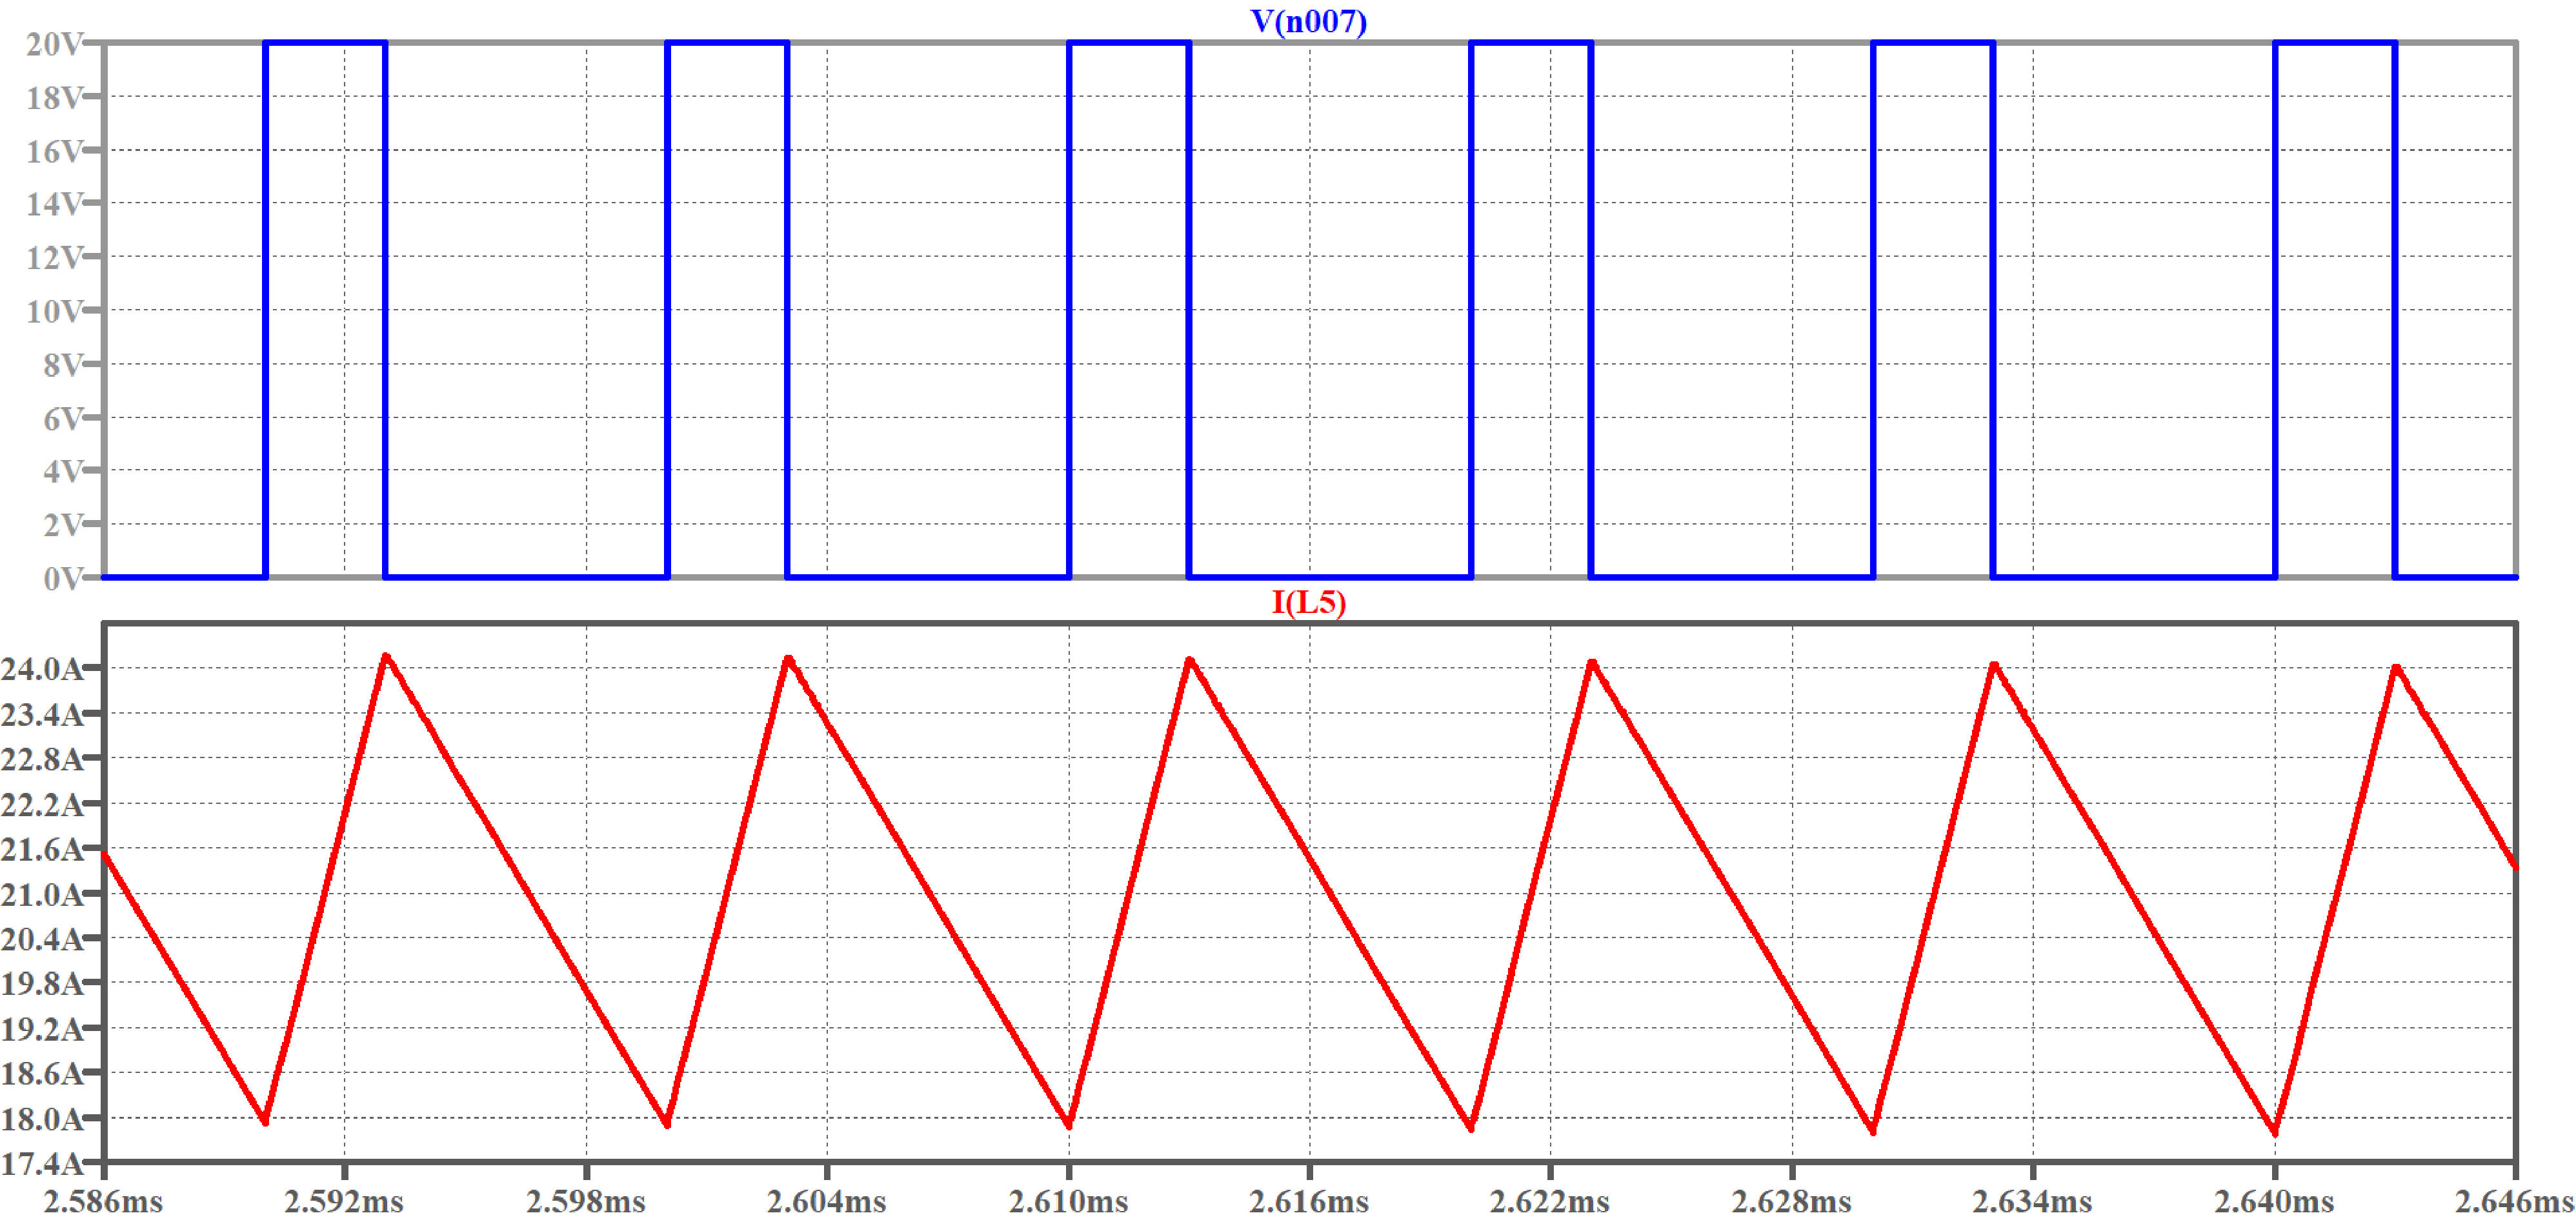
\includegraphics[width=0.8\linewidth]{Pictures/Images/LT_inductor_current.pdf}
    \caption{\textcolor{blue}{\textit{\footnotesize Duty Cycle and Inductor Current Wave Form}}}
\end{figure}